\documentclass{book}
\usepackage{graphicx} % Required for inserting images

\usepackage[utf8]{inputenc}
\usepackage[T1]{fontenc}
\usepackage{listings}
\usepackage{appendix}
\renewcommand{\lstlistingname}{Algoritmus}

\title{Avances de tesis}
\author{r.reyes }
\date{December 2023}

\begin{document}

\maketitle

\tableofcontents

\newpage

\chapter{Introducción}

En el medio interestelar hay muchas cosas maravillosas que nos permiten entender mucho acerca de la física en las diferentes regiones que observamos.

Las estrellas se forman a partir del colapso gravitacional en nubes moleculares frías, teniendo sus diferentes fases durante este proceso, algunas regiones en las que se pueden formar son en lo que llamamos \textit{glóbulos de Bok}, que son nubes oscuras, relativamente pequeñas si las comparamos con otras regiones de formación estelar, que tienen una gran cantidad de gas y polvo. Estas nubes fueron observadas por primera vez por el astrónomo Bart Bok en 1940. 

Estos glóbulos contienen principalmente hidrógeno molecular en su interior, así como también puede tener otras moléculas, metales e incluso algunos silicatos. Si bien pueden tener formación estelar en su interior, no podemos ver la radiación UV ya que esta es absorbida por el hidrógeno atómico y el polvo, es por eso que se ven oscuras. Sin embargo, estos pueden ser radiados externamente, en regiones de formación estelar, por estrellas jóvenes que se están formando cerca, y si la radiación es lo suficientemente fuerte, en algunos casos podemos ver el frente de ionización. Gracias a estas interacciones podemos ver que se forman estructuras como columnas, dedos o pilares en estas nubes

Esta interacción se puede dar a diferentes escalas, por lo que se les puede conocer con diferentes nombres según la escala. Por ejemplo en Cygnus OB2, que es una de las regiones se mayor formación estelar, vemos que la interacción de estos glóbulos puede alcanzar tamaños de hasta 1 pc. También se ha observado a escalas más pequeñas, como en regiones H II. 

Esto también se puede dar en nebulosas planetarias, donde se les conoce también como nudos. Aquí vemos que la escala física es mucho más pequeña que en los glóbulos de Bok. 

\section{Flujos de foto evaporación ionizada}

Como ya mencionamos hay muchos tipos de glóbulos de diferentes tamaños, en diferentes regiones. Algunos más pequeños que otros. 

En nuestro caso nos concentraremos en lo que llamaremos \textit{nudos}, los cuales se encuentran principalmente en nebulosas planetarias, estos son glóbulos de un tamaño relativamente pequeño y tiene una gran concentración molecular neutra. Debido a la radiación UV de la estrella central esta comienza a ser ionizada en la superficie más cercana a la estrella. ...
%Lyman continuo, proceso intermedio
Después de cierto tiempo, podemos llegar a un equilibrio de ionización, donde esta superficie cercana a la estrella es ionizada por el continuo de Lyman, mientras que también tenemos procesos de recombinación. Estas recombinaciones de en la superficie de los nudos pueden emitir intensamente ...

\section{Estrellas Wolf-Rayet y sus vientos}

\section{Nebulosa M1-67}

Gracias a las nuevas imágenes de JWST podemos saber mejor como es la nebulosa M1-67 que rodea la estrella WR-124. En setas imágenes vemos como la nebulosa es muy simétrica en algunos filtros, mientas que en algunos otros la emisión de los diferentes mecanismo se ven más intensos de un lado que del otro.

Algo muy notorio a simple vista es que tiene una simetría que...

%Poner imagen de M1-67

Podemos ver como muchos detalles en cada uno de los filtros, en especial de como podemos ver en color rosa lo que parece ser choques de una gran acumulación de gas neutro que está interactuando con el viento de la estrella, y al rededor de ellos vemos una morfología similar a la de los proplyds que hay en otras nubes moleculares. También podemos ver como estos tienen una estela en la parte más lejana de la interacción, pero para nuestro estudio solo nos concentraremos solo en la parte más central.

\chapter{Modelos analíticos de flujos foto evaporativos interactuando con una presión externa}

En este capitulo vamos  describir nuestro modelo, esto con el fin de explicar la interacción que hay entre el flujo foto evaporativo de unos glóbulos, que es provocado por la radiación de una estrella, y el viento estelar, que proviene de la misma estrella. Tomaremos estos glóbulos separados unos de otros, por lo que comenzaremos por describir la interacción del flujo foto evaporativo de un solo glóbulo y el viento estelar.

Para nuestro modelo estamos considerando que los glóbulos contienen principalmente hidrógeno neutro y tienen una forma esférica. Estos glóbulos deben estar lo suficientemente cerca de una estrella masiva como para que su radiación UV pueda ionizar el hidrógeno que hay en la superficie de estos glóbulos. Esta interacción con la radiación UV de la estrella hace que tengamos un flujo foto evaporativo súper sonico que sale de la superficie del glóbulo. Este flujo foto evaporativo estará interactuando con el viento estelar que proviene de la misma estrella de la cual esta recibiendo la radiación UV. En esta interacción tenemos un choque interno y uno externo, así como una discontinuidad de contacto como se ve en la siguiente figura.

\begin{figure}[h]
    \centering
    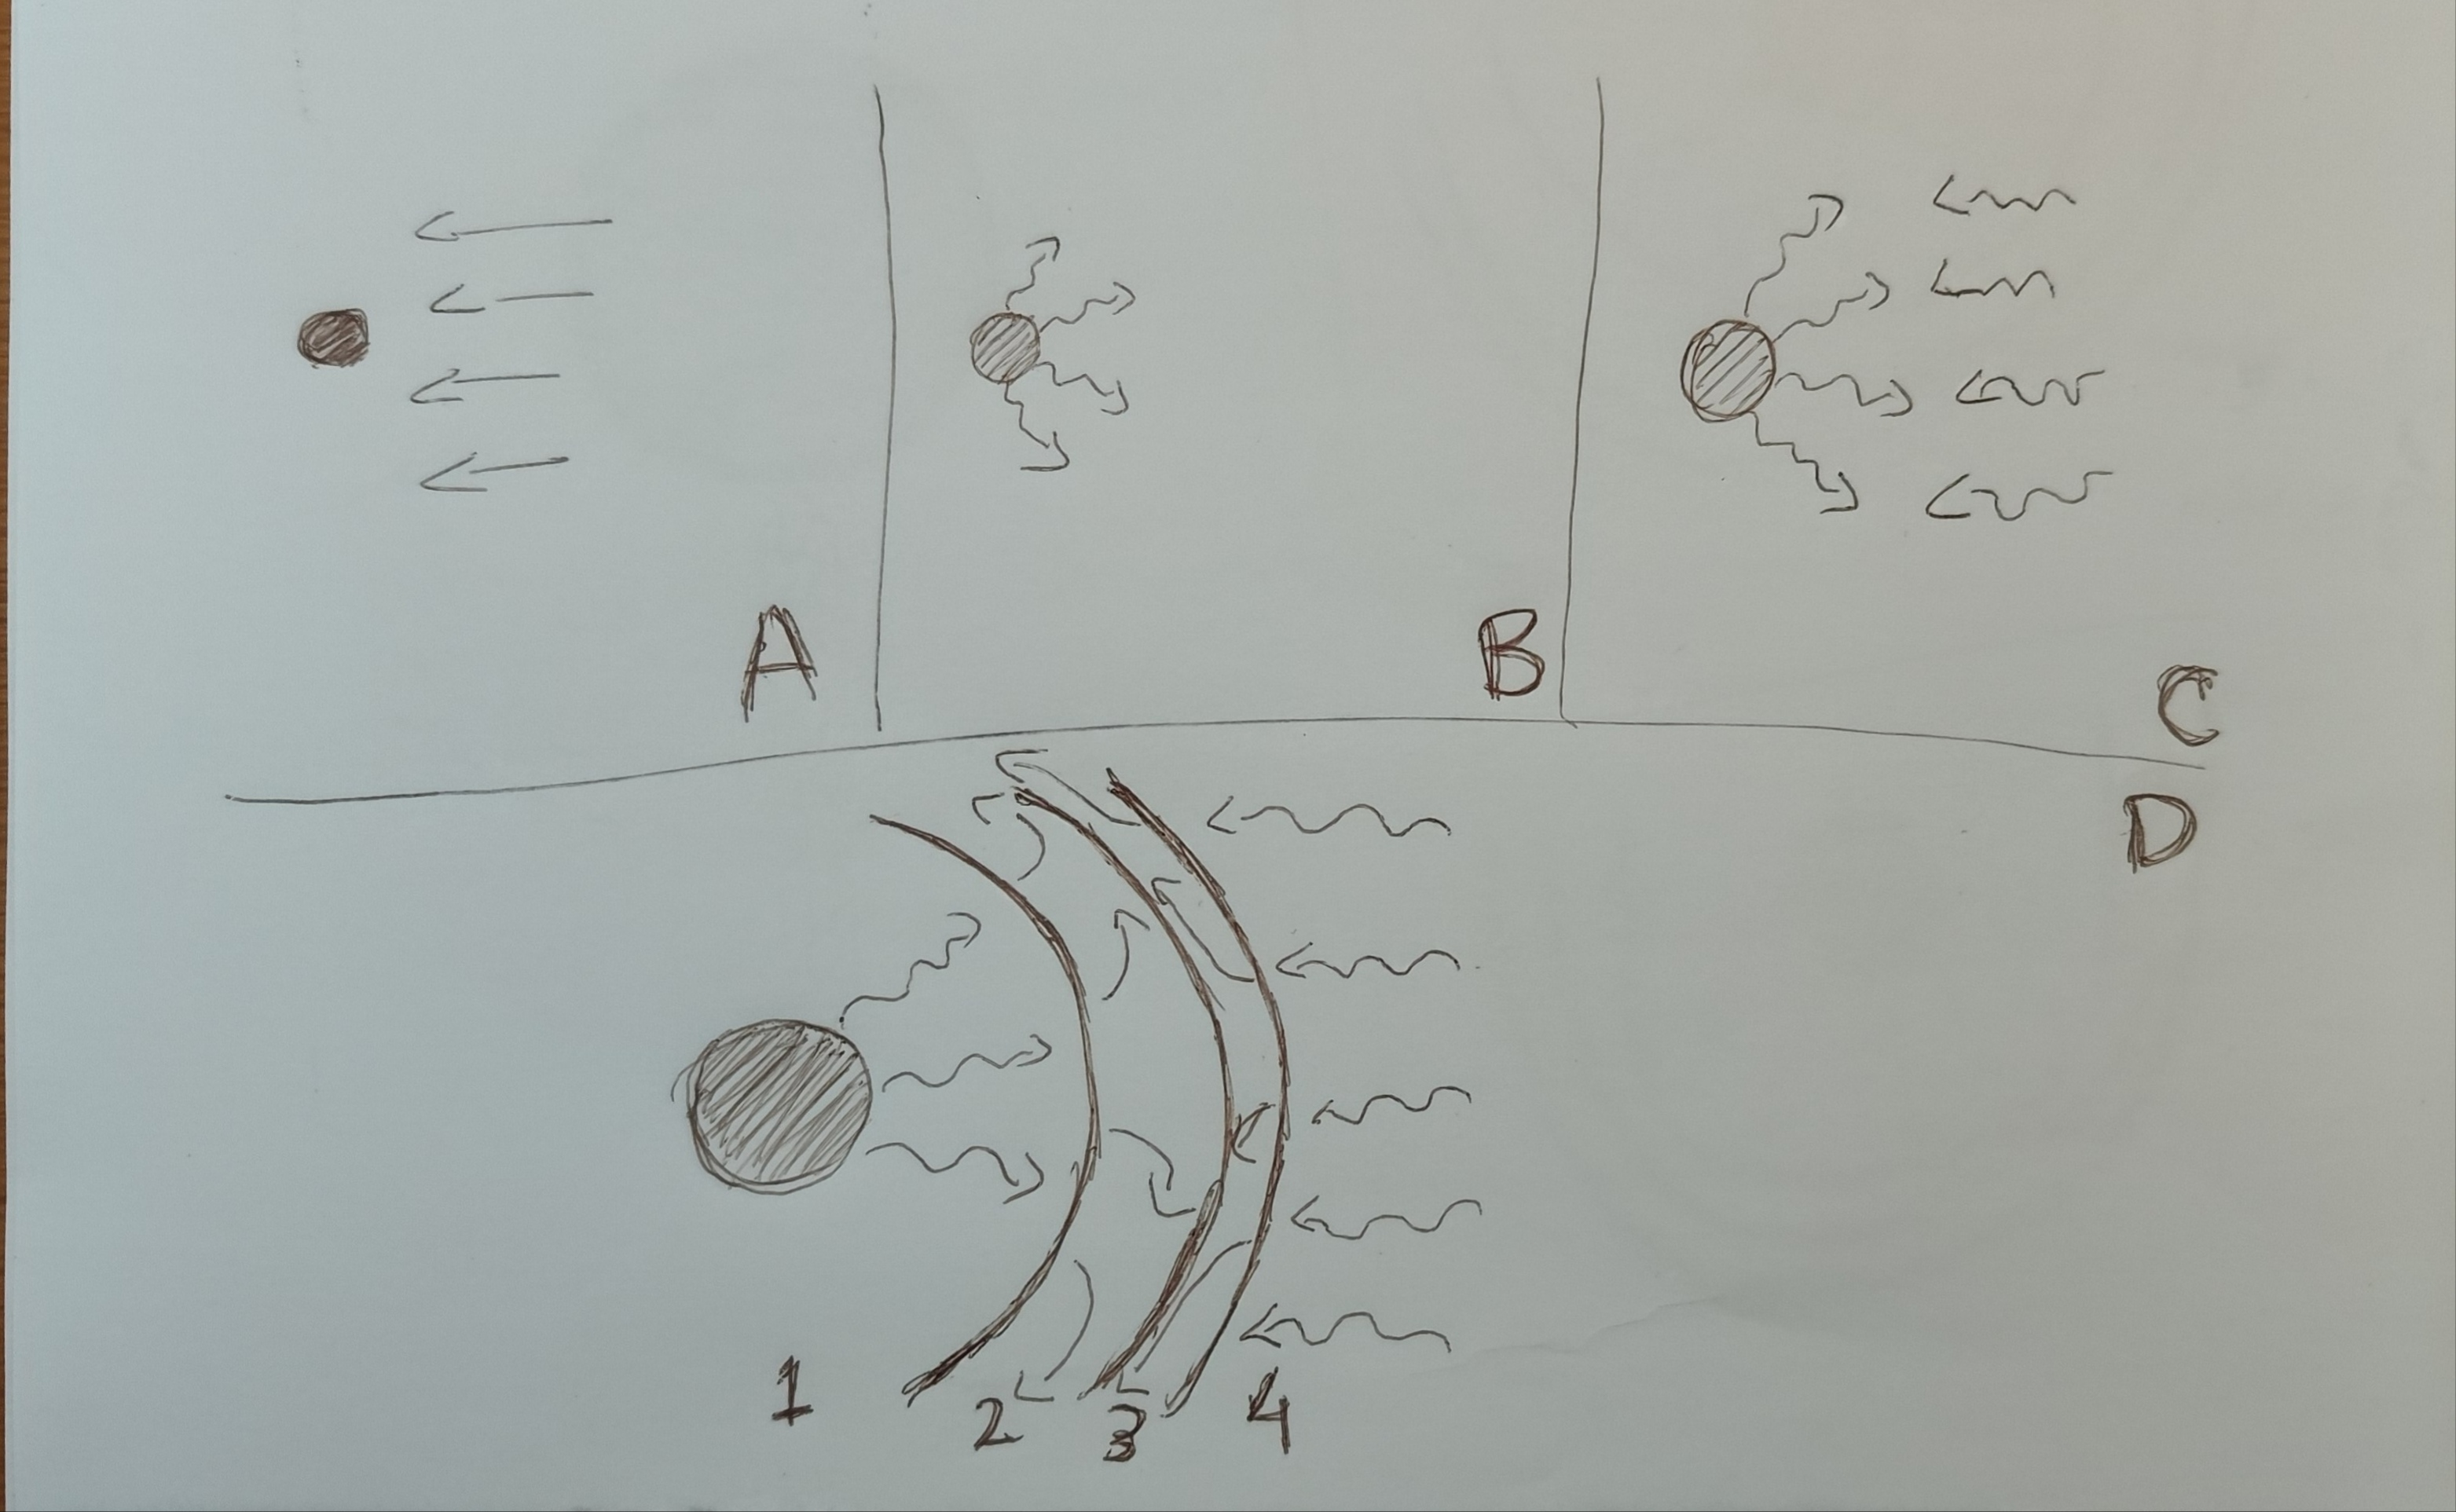
\includegraphics[width=0.75\textwidth]{Chp2_zones.jpg}
    \caption{En \textbf{A} vemos como la radiación UV por parte dela estrella incide en el glóbulo. En \textbf{B} vemos como después de esta interacción comienza a salir el flujo foto evaporativo de la superficie del glóbulo. En \textbf{C} vemos la interacción entre el flujo fotoevaorativo y el viento estelar por parte de la estrella. Finalmente en \textbf{D} vemos las diferentes regiones que se forman en la interacción en \textbf{C}, la  región 1 es donde el flujo foto evaporativo sale de la superficie del glóbulo inicialmente con un número de Mach de 1 y se va haciendo super sónico, en la región 2 es la parte del flujo foto evaporativo chocado, la cual esperamos ver en las observaciones. La región 3 es el viento estelar chocado, esta región suele ser muy delgada en comparación con la región 1 y como es mucho menos denso que la región 2, podría no verse observacionalmente. Entre las regiones 2 y 3 tenemos una discontinuidad de contacto. La región 4 es la parte del viento estelar, la cual tiene una densidad baja comparada con la del flujo fotoevaporativo}
    \label{fig:zones}
\end{figure}

La interacción entre el flujo fotoevaporativo y el viento estelar puede ser diferente morfológicamente, dependiendo si el flujo fotoevaporativo es isotópico o anisótropo. Por lo que en un principio vamos a tratar este problema de manera radial con una simetría cilíndrica en la cual consideraremos un ángulo preferencial, de esta manera lo trataremos como un problema unidimensional.

\begin{figure}[h]
    \centering
    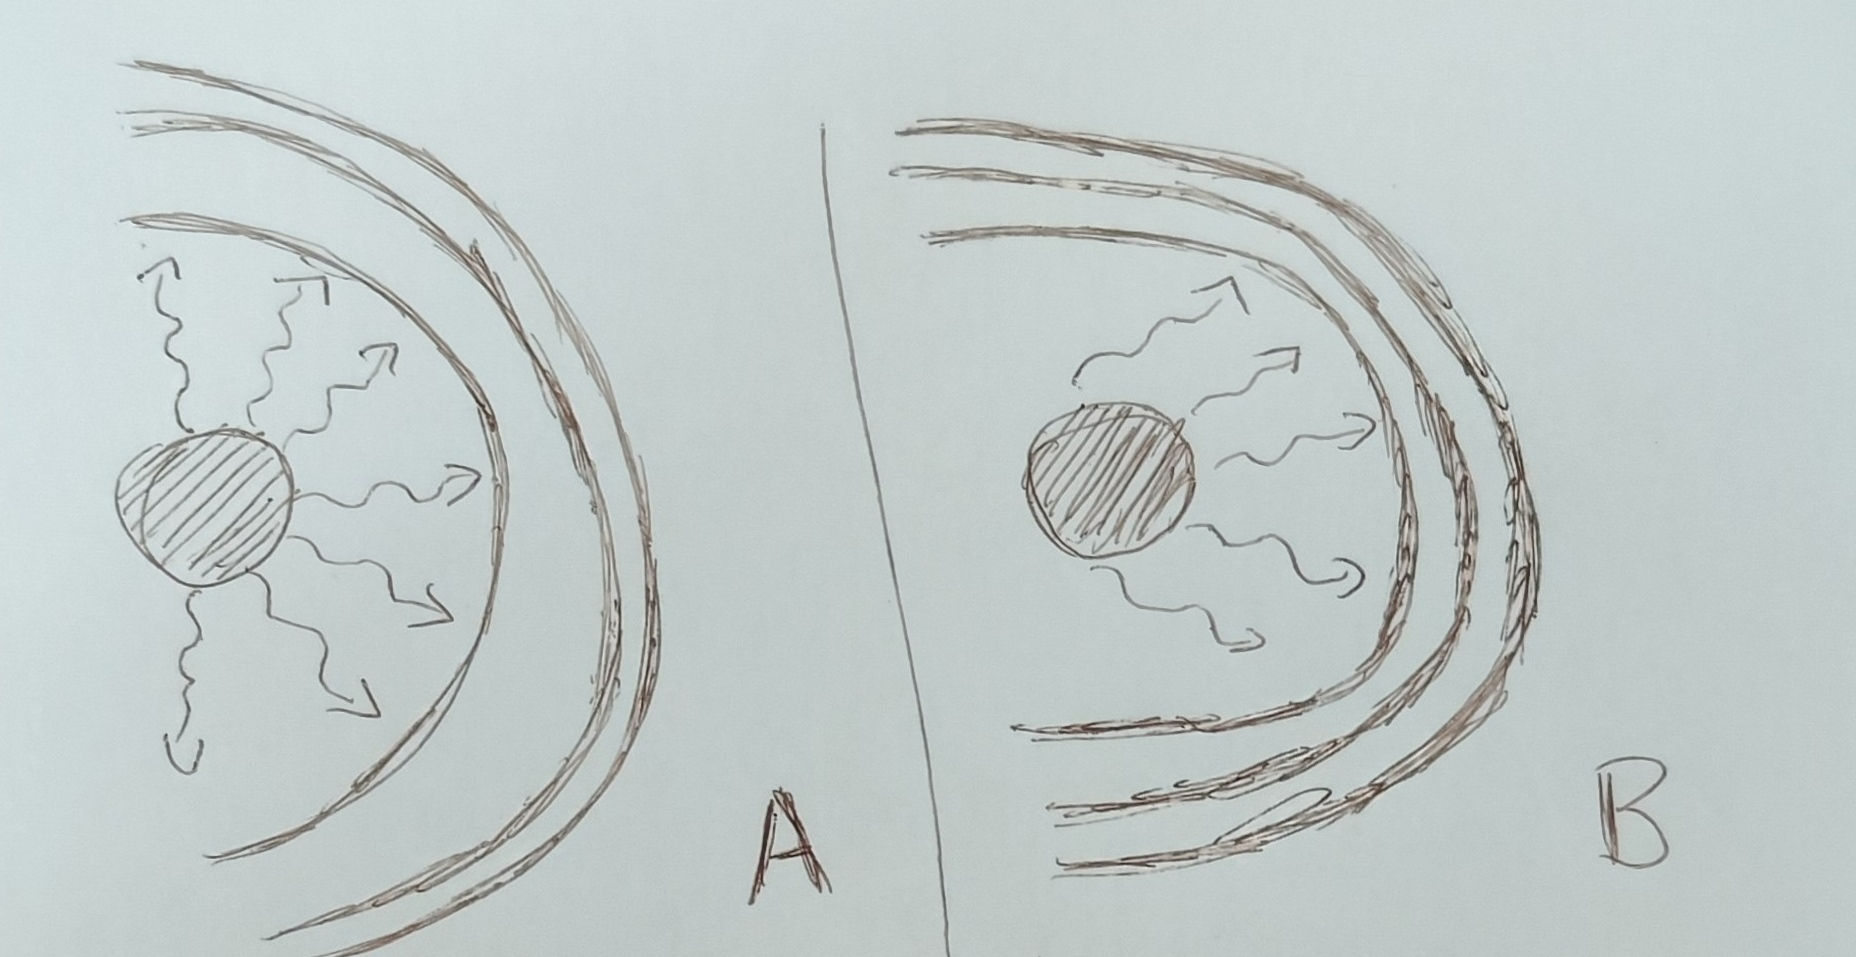
\includegraphics[width=0.75\textwidth]{Chp2_iso&ans.jpg}
    \caption{\textbf{A} es la interacción de un fujo fotoevaporativo isotópico con un viento externo y \textbf{B} es la interacción de un flujo fotoevaporativo anisótropo con un viento externo. Vemos que en el caso isotópico se nos es más fácil tratar las diferentes regiones de manera radial debido a la geometría.}
    \label{fig:isotyaniso}
\end{figure}

Dado que el flujo fotoevaporativo es más denso que el viento estelar, esperamos ver solo el flujo fotoevaporativo chocada y no el viento estelar chocado.

\begin{figure}[h]
    \centering
    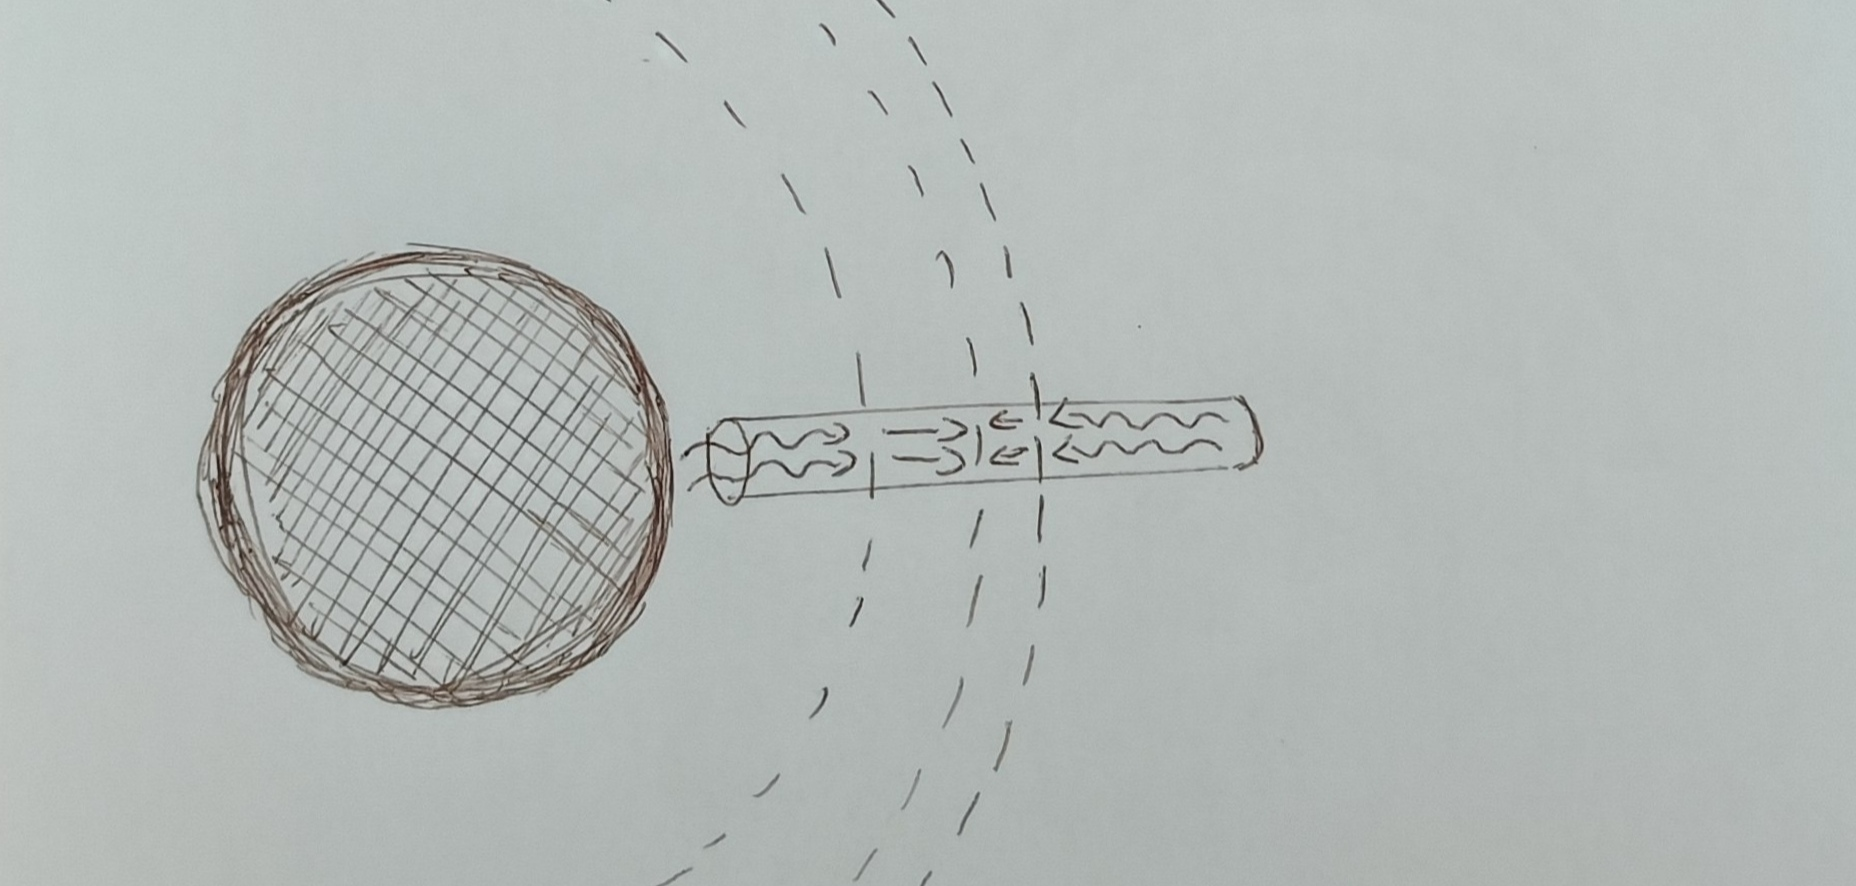
\includegraphics[width=0.75\textwidth]{Chp2_cilinders.jpg}
    \caption{Si consideramos una simetría cilíndrica con un radio muy pequeño, podemos tratar este problema de manera radial y de tal manera que la radiación y el viento estelar inciden de manera perpendicular al glóbulo.}
    \label{fig:cilinders}
\end{figure}

\section{Estimación de la densidad ionizada a partir del brillo superficial de $H_\alpha$}

Para estimar la densidad ionizada, usamos primero la definición de medida de emisión (EM por sus siglas en inglés)
\[EM=\int_z n_in_edz\] donde en este caso estaremos integrando sobre nuestra línea de visión. Esta EM depende tanto de la densidad de electrones como de iones, pero en nuestro caso vamos a considerar un equilibrio de ionización entre el flujo foto evaporativo y el viento estelar, por lo que $n_e=n_i$.

Si suponemos una simetría esférica entre esta interacción del flujo fotoevaporativo y el viento estelar, podemos tomar, por geometría, que
\[EM=2\sqrt{rh}n^2.\]

%Insertar imagen de los radios

Esto ya que de la fig(?) tenemos que por geometría $r^2+\frac{1}{2}l^2=(r+h)^2=r^2+2rh+h^2\approx r^2+2rh\Rightarrow l=2\sqrt{rh}$, por lo que podemos estimar la densidad ionizada a través de la EM como \[n=\sqrt{\frac{EM}{l}}\]

\section{Modelo hidrodinámico estacionario}

Para el caso de nuestro modelo analítico consideraremos un modelo analítico hidrodinámico estacionario, esto ya que consideramos que la interacción entre el flujo foto evaporativo y el viento estelar ha llegado al equilibrio de ionización.

%inseratr imagen de las regiones durante la interaccion
.

Para este modelo consideramos glóbulos relativamente pequeños, de unos 200-300 mili arco segundos de diámetro comparado con su entorno que puede ser unas pocas decenas de arco segundos, además a unos 10-30 arco segundos de la estrella masiva como para que su radiación UV llegue desde un pequeño ángulo e interactúe con el glóbulo, de esta manera podemos decir que la radiación incide perpendicularmente a la superficie del glóbulo.

En nuestro caso tomamos una simetría cilíndrica en la cual podamos tomar un radio perpendicular de un tamaño muy pequeño como para tomar este problema solo de manera radial, pero notemos que debido a la forma de estos glóbulos, en realidad tendremos una familia de cilindros a cada ángulo, por lo que tomando el radio perpendicular a la radiación muy pequeño, entonces podemos considerar este problema solo de manera radial, un problema unidimensional, en la dirección en la que incide la radiación de la estrella.

En general en el medio interestelar hay muchas fuerzas que afectan el cambio en la materia, pero en este caso vamos a despreciar la fuerza de gravedad, tanto del mismo glóbulo como la gravedad impuesta por la estrella, tampoco vamos a considerar fuerza por campos magnéticos por simplicidad. Por lo que solo vamos a considerar las fuerzas dada por el gradiente de presión por parte del flujo fotoevaporativo, donde tomaremos el viento estelar como condición de frontera.

Para el flujo fotoevaporativo por parte del glóbulo vamos a considerar las ecuaciones de hidrodinámica, la ecuación de conservación de masa ya que como dijimos antes, el tiempo en el que un bulto sale de esta interacción le toma bastante tiempo. Usaremos también la ecuación de Bernoulli para un gas isotermo, donde la velocidad del sonido en este gas dependerá de la temperatura.

% Balance between ionizations and recombinations

\section{Ecuación de estado y equilibrio de ionización}

Para nuestro flujo tomaremos dos presiones, la hidrodinámica y la térmica, por lo que tenemos una presión total dada por
\[P_{tot}=P_{ter}+P_{hid}=n\bar{m}c_s^2+n\bar{m}u^2=\rho c_s^2(1+M^2)\]

En nuestro modelo consideramos que nuestro flujo que sale de la base del glóbulo tiene como condiciones iniciales
\[M=1\]
\[r=r_0\]
\[\rho=\rho_0\]
\[P_{tot}=P_0\]
y en nuestro modelo queremos ver cuando la presión del flujo llega a un equilibrio con la presión RAM del viento estelar, por lo que queremos conocer a que distancia se da, $r_1$, y que densidad y número de Mach tendría, para esto vamos a tomar que la presión disminuyó una fracción de la presión inicial. Por lo que la presión cambia como 
\[\frac{P}{P_0}=\frac{\rho c_s^2(1+M^2)}{\rho_0 c_s^2(1+1)}=\frac{\rho}{\rho_0}\frac{1+M^2}{2}\]
Considerando la ecuación para la conservación de masa tenemos que
\[\rho r^2M	=\rho_0 r_0^2\]
y finalmente si consideramos la ecuación de Bernoulli isotérmica 
\[\dots\]
de la cual tenemos 
\[\frac{r}{r_0}=M^{-1/2}e^{\frac{M^2-1}{4}}\]
Ahora que tenemos tres ecuaciones y tres incógnitas podemos resolver, en nuestro caso lo hicimos de manera numérica. Al resolver estas ecuaciones para diferentes $f$ tenemos que tanto la presión como la densidad decaen con el radio, mientras que el número de Mach aumenta.

%Imagen temporal de como depende la densida, presio y M como funcion del radio 



% Assumption of isothermal equation of state

% General solution for the internal structure of model


\chapter{Aplicación a M1-67}

\section{Observaciones con HST}

\section{Observaciones con JWST}

\section{Ajustando el modelo a los perfiles de brillo radial}

\section{Estimando la presión RAM del viento estelar}

\section{Estimando la tasa de foto ionización}

\chapter{Conclusiones}

\appendix
\chapter{Estimación de fuerzas en el modelo}
\end{document}
